\chapter{Application to electron-phonon systems}

\section{Non-interacting phonon system and Debye theory of specific heat}

\begin{wrapfigure}{l}{5.5cm}
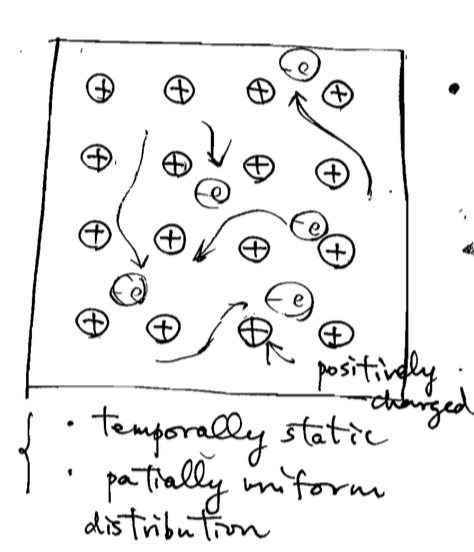
\includegraphics[width = 5cm]{5-1.png}
\end{wrapfigure}

In a usual metal, such as alkali metals of column I, outer shell valence electrons are completely separated from their ion cores and form a nearly free electron gas. 

In the section 1-8, we have treated the positively charged ion cores as temporally-static and uniformly-distributed positively-charged background. 

Thereby, the only play role of ensuring the electrical neutrality of the whole system. 

In this section, we will study the dynamics of the positively charged backgrounds, and their effect on the electron gas. 

In real metals, the ionic background form a lattice structure, so that it is not exactly the uniformly distributed positive charges. 

But, when it comes to the acoustic mode, in which all the ion cores are moving in the same `phase', the discreet lattice structure is irrelevant and we can treat them as a positively charged continuous elastic media. 

To describe the acoustic wave, let us first define a three-dimensional vector field $\bm d$ as a function of the spatial coordinate $\bm x$, which we call displacement vector:

\[\bm{d}(\bm{x}):\quad\text{displacement vector} \]

Physically, $\bm{d(x)}$ denotes how the ionic core at position $\bm x$ is displaced:

\[\bm{u(x) - \langle u(x)\rangle \equiv d(x)} \]

Compared to the displacement field $\varphi$ introduced in section 1-4, such a quantity is characterized by three component real-valued vector in a $3$-dimensional elastic media

\[\bm{d(x) = (d_1(x),d_2(x),d_3(x))} \]

According to the Helmholtz-Hodge's decomposition theorem, any vector field in $3$0dimensional space can be decomposed into divergence-free vector and a rotation-free vector

\[\bm{d(x)} = \nabla\phi + \nabla\times\vec{\bm{A}} \]

Although we always have ambiguity when decomposing into the two, let us temporally denote the rotation-free part as $\bm{d'(x)}$ and the divergence-free parts as $\bm{d''(x)}$ so that

\[\begin{cases}
\nabla\times\bm{d'} = 0\\
\nabla\cdot\bm{d''} = 0
\end{cases}\]

Corresponding to this decomposition, the acoustic waves are composed of two different kinds. 

One is called the longitudinal acoustic wave, which is described only by the rotation-free vector field $\bm{d'}$ (To be precise, $\nabla\cdot \bm{d'} = \nabla\cdot\bm{d}$): longitudinal(compressional) acoustic wave. 

The other is called the transverse acoustic waves, which are described only by the divergence-free part $\bm{d''}$ (to be precise, $\nabla\times\bm{d''} = \nabla\times\bm{d}$): transverse(shear) acoustic waves. 

$\nabla\cdot \vec{\bm{d}}$ is nothing but the charge density modulation in a positively charged background

\[\nabla\cdot\vec{\bm{d}} = -\frac{\delta\rho_{inoic}}{\rho_0}\]

\begin{wrapfigure}{l}{5.5cm}
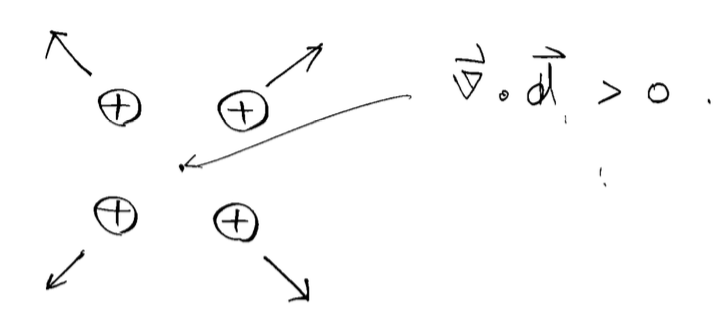
\includegraphics[width = 5cm]{5-2.png}
\end{wrapfigure}
One can easily see this, by drawing a configuration of the displacement vector, which has a finite divergence. 

Namely, when these ionic charges are displaced like in this picture, we have effectively a negative charge in the middle. 

On the one hand, $\nabla\times\bm{d}$ is accompanied by the shear deformation in the positively charged ionic background, e.g.,

\begin{figure}
\end{figure}
\begin{wrapfigure}{l}{6.5cm}
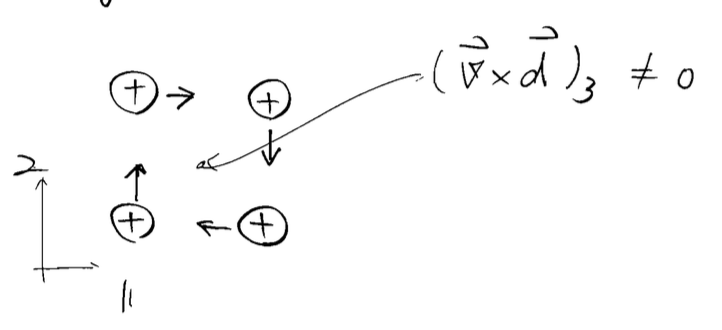
\includegraphics[width = 6cm]{5-3.png}
\end{wrapfigure}

which is not accompanied by any charge density modulation. 

Since electrons and positively charged background are coupled with each other by electrostatic Coulomb interaction, we usually regard that the longitudinal acoustic waves are strongly coupled with electrons, while the transverse waves are not. 

For this reasoning, we will focus only on the longitudinal (compressional) acoustic wave, where we enforce the displacement vector is rotation-free

\[\nabla\times\vec{\bm{d}}(\bm{x},t) = 0,\forall\bm{x},t \]

In order to introduce the equation of motion for the charge density modulation

\[\nabla\cdot\vec{\bm{d}}(\bm{x},t) = \delta\rho_{ion}(\bm{x},t) \]

Let us begin with the Newton's equation of motion for a fluid element

\[\frac{D\vec{p}}{Dt} = \vec{f} \]

Here $\bm{p}(\bm{x},t)$ is the momentum density field at position $\bm{x}$ at a given time $t$ which is given by a product between mass density field and velocity field

\[\bm{p}(\bm{x},t) = \rho(\bm{x},t)\bm{v}(\bm{x},t) \]

The temporal derivative in the right hand side is a Legendre derivative often used int the course of fluid mechanics. 

\[\frac{D\bm{p}}{Dt} \overset{def}{\equiv}\lim_{\Delta\rightarrow0}\frac{1}{\Delta t} \left\{\bm{p}(\bm{x}+\bm{v}\Delta t,t+\Delta t) - \bm{p}(\bm{x},t)\right\} = \frac{\partial\bm{p}}{\partial t}+(\bm{v}\cdot\nabla)\bm{p} \]

The force acting on the fluid element is a restoring force which comes from the spatial gradient of the pressure:

\[\frac{\partial}{\partial t}(\rho\bm{v})+(\bm{v}\cdot\nabla)(\rho\bm{v}) = -\nabla P \]

In the equilibrium, we don't have any velocity field and the mass density is uniformly distributed and static

\[\left.\begin{split}
\rho(\bm{x},t) &= \rho_0\\
\ & \ \\
\bm{v}(\bm{x},t) &= 0
\end{split}\right\}\text{\quad equilibrium} \]

Out of the equilibrium, we have finite velocity field and mass density is spatially and temporally dependent:

\[\left.\begin{split}
\rho(\bm{x},t) &= \rho_0 + \delta\rho(\bm{x},t)\\
\ & \ \\
\bm{v}(\bm{x},t) &\neq 0
\end{split}\right\}\text{\quad out of equilibrium} \]

When linearizing this equation of motion for a small derivation from the equilibrium, we can regard that the $2^{\text{nd}}$ term in the right hand side is the $2^{\text{nd}}$ order in $\delta\rho$ and thus negligible:

\[\frac{\partial}{\partial t}\left((\rho_0+\delta\rho)\bm{v}\right) + (\bm{v}\cdot\nabla)\left((\rho_0+\delta\rho)\bm{v}\right) = -\nabla P \]

\[\rho_0\frac{\partial\bm{V}}{\partial t} + {\color{red}{O((\delta\rho)^2)}}= -\nabla p \]

,\footnote{The red part is omit-able. }

In addition to this Newton's equation of motion, the mass density field and velocity field must satisfy the continuity equation: 

\[\frac{\partial \rho}{\partial t}+\nabla\cdot(\rho\bm{v}) = 0 \]

When linearized with respect to a small $\delta \rho$, we have

\[\frac{\partial\delta\rho}{\partial t} = -\rho_0(\nabla\cdot\bm{v}) \]

Combining these two linearized equation, we have

\[\frac{\partial^2\delta\rho}{\partial t^2}= -\rho_0(\nabla\cdot\frac{\partial\vec{\bm{v}}}{\partial t}) = \nabla^2 P \]

A pressure of a given fluid element is determined by the mass density of the element, so that it is quite natural to assume that the pressure depends on the spatial coordinate $\bm{x}$ only through $\rho$. 

\[\nabla^2 P = \nabla^2 P(\rho_0+\delta\rho(\bm{x},t),\cdots) \approx\left(\frac{\partial P}{\partial\rho}\right)_{\rho_0}\nabla^2\delta\rho \]

This leads to the following closed equation of motion for the density fluctuation:

\[\frac{\partial^2\delta\rho}{\delta t^2} = \left(\frac{\partial P}{\partial \rho}\right)_{\rho_0}\nabla^2\delta\rho \]

For many elastic continuous media, we can define (adiabatic) bulk modulus. 

\[\begin{split}
B &= -B\left(\frac{\partial O}{\partial V}\right)_{equilibrium}\\
&\quad\quad \rho = \frac{M}{V},\ \quad \frac{d\rho}{dV} = M\left(-\frac{1}{V^2}\right)\\
&= -V\left(\frac{\partial P}{\partial\rho}\right)M\left(-\frac{1}{V^2}\right)\\ &= \frac{M}{V}\left(\frac{\partial P}{\partial \rho}\right)_{eq} \overset{def}{\equiv}\rho_m\left(\frac{\partial P}{\partial\rho}\right)_{eq}
\end{split} \]

In terms of the bulk modulus, the coefficient of the right hand side is given by 

\[\frac{\partial^2\delta\rho}{\partial t^2} = \frac{B}{\rho_m}\cdot\nabla^2\delta\rho \equiv c^2\nabla^2\delta_\rho \]

Here $c$ is nothing but a velocity, with which the density fluctuation propagates in space as time passes by, and which is often called as the ``sound velocity'' of the longitudinal acoustic wave. 

As explained already, the density fluctuation is given by the divergence of the displacement field, the equation of motion for the displacement field is given by 

\[\frac{\partial}{\partial t}(\nabla\cdot\vec{\bm{d}}) = c^2\nabla^2(\nabla\cdot\vec{\bm{d}}) \]

\[\nabla\cdot\left(\frac{\partial \vec{\bm{d}}}{\partial t} - \nabla^2\vec{\bm{d}}\right) = 0 \]

Remember again that we are interested only in the longitudinal acoustic wave, so that the displacement field is rotation free at any space and time. 

\[\nabla\times\vec{\bm{d}} \equiv\vec{0} \]

The latter condition ensures that

\[\nabla\times\left(\frac{\partial \vec{\bm{d}}}{\partial t} - \nabla^2\vec{\bm{d}}\right) = 0\]

because $\nabla\times$ and $\partial_t$ or $\nabla^2$ commute with each other. 

From these two, we have a pair of equation which is satisfies by the displacement field $\bm{d}$. 

\[\begin{cases}
\frac{\partial\bm{d}}{\partial t} - c^2\nabla^2\bm{d} &= 0\\
\ &\ \\
\nabla\times\bm{d} &= 0
\end{cases}\]

So far, we just describing a classical equation of motion for the displacement field; in order to second-quantize this classical field, let us first introduce the Lagrangian which leads to this equation of motion:

\[L_0 = \frac{1}{2}\sum_{i,j=1,2,3}\int d^3\bm{x}\int dt\left[\rho_m\frac{\partial d_i}{\partial t}\cdot\frac{\partial d_i}{\partial t} - B\frac{\partial d_i}{\partial x_j}\frac{\partial d_i}{\partial x_j}\right]\]

Notice that

\[\int \left[\rho_m\frac{\partial d_i}{\partial t}\cdot\frac{\partial d_i}{\partial t} - B\frac{\partial d_i}{\partial x_j}\frac{\partial d_i}{\partial x_j}\right] = \delta L_0\]
\[\rho_m\delta d_i\left[\frac{\partial^2 d_i}{\partial t^2} - c^2\sum_{j = 1,2,3}\frac{\partial^2 d_i}{\partial x_j^2}\right] = \delta L_0 \]

Under the $2$nd condition of rotation-free, the Lagrangian can be rewritten into the following:

\[L_0 = \frac{1}{2}\sum_{i,j}\int d^3\bm{x}\int dt \left[\rho_m\frac{\partial d_i}{\partial t}\cdot\frac{\partial d_i}{\partial t} - B\frac{\partial d_i}{\partial x_i}\frac{\partial d_j}{\partial x_j}\right] (=\int dt \tilde{L}_0) \]

To see this, let us begin with the following identity:

\[(\nabla\times\vec{d})\cdot(\nabla\times\vec{d}) = 0 \]

\[\epsilon_{ijk}\partial_j d_k\epsilon_{ilm}\partial_l d_m = 0 \]

\[(\delta_{il}\delta_{km} - \delta_{jm}\delta_{kl})\partial_j d_k\partial_l d_m = 0 \]

\[\sum_{i,j = 1,2,3} \partial_j d_i \partial_j d_i - \sum_{i,j}\partial_j d_i \partial_i d_j = 0 \]

Under the space integral, we can take a partial integral of the $2$nd term in the left hand side

\[\sum_{i,j}\int d^3{\bf x}[\partial_j d_i\partial_j d_i+(\partial_j\partial_i d_i)d_j] = 0 \]

\[\sum_{i,j}\int d^3{\bf x}[(\partial_j d_i)(\partial_j d_i) - (\partial_i d_i)(\partial_j d_j)] = 0 \]

The final identity allows us to rewrite this into this

\dotfill

\ 

So far, we have treated the classical action. To second-quantize this classical degree's of freedom, we follow the exactly the same procedure we formulated in chapter 1. 

Namely, we first introduce a momentum variable which is conjugate the displacement field

\[\Pi_j = \frac{\delta L_0}{\delta \dot{d}_j} = \rho_m\dot{d}_j \]

Or equivalently 

\[\tilde{\Pi}_j\equiv\frac{1}{\sqrt{\rho_m}}\Pi_j,\quad \tilde{d}_j\equiv\sqrt{\rho_m}d_j \]

with 

\[\tilde{\Pi}_j = \frac{\delta L_0}{\delta\dot{\tilde{d}}_j} = \dot{\tilde{d}}_j \]

Then the Hamiltonian is given by 

\[\begin{split}
H_0 &= \int d^3{\bf x}\tilde{\Pi}_j\dot{\tilde{d}}_j - \tilde{L}_0\\
 &=\frac{1}{2}\int d^3{\bf x}\tilde{\Pi}_j({\bf x})\tilde{\Pi}_j({\bf x}) + \frac{1}{2}\int d^3{\bf x}\frac{B}{\rho_m}(\nabla\cdot\tilde{\bf d}{\bf(x)})^2\\
 & \quad\quad\quad\quad\quad\quad\quad\quad\quad\quad\quad\quad\quad\quad\quad \frac{B}{\rho_m} = c^2
\end{split}\]

To quantize these field operators we suppose that $\tilde{\bf d}(\bf x)$ and $\tilde{\Pi}(\bf x)$ are hermite operators, which satisfy the following commutation relation

\[[\tilde{\Pi}_j({\bf x}),\tilde{\Pi}_m({\bf x'})] = [\tilde{\bf d}_j({\bf x}),\tilde{\bf d}_m({\bf x'})] = 0 \]

\[[\tilde{\bf d}_j({\bf x}), \tilde{\Pi}_m({\bf x'})] = i\hbar\delta_{jm}\delta^3(\bf x-x') \]

As we did in the chapter 1, it is much useful to introduce their Fourier series:

\[\begin{cases}
\tilde{\bf d}_j({\bf k}) &= \displaystyle\int d^3{\bf x}\tilde{\bf d}_j({\bf x}) e^{-i\bf k\cdot x}\\
\ & \\
\tilde{\Pi}_j({\bf k}) &= \displaystyle\int d^3 {\bf x} \tilde{\Pi}_j({\bf x}) e^{-i\bf k\cdot x}
\end{cases}\]

where the inverse is

\[\begin{cases}
\tilde{\bf d}_j({\bf x}) &= \displaystyle\int d^3{\bf k}\tilde{\bf d}_j({\bf k}) e^{i\bf k\cdot k}\\
\ & \\
\tilde{\Pi}_j({\bf x}) &= \displaystyle\int d^3 {\bf k} \tilde{\Pi}_j({\bf k}) e^{i\bf k\cdot k}
\end{cases}\]

Since $\tilde{\bf d}_j({\bf x})$ \& $\tilde{\Pi}_j({\bf x})$ are both Hermite operators, we have

\[\begin{cases}
\tilde{\bf d}_j({\bf k}) &= \tilde{\bf d}_j({-\bf k})\\
\ & \\
\tilde{\Pi}_j({\bf k}) &= \tilde{\Pi}_j(-\bf k)
\end{cases}\]

In terms of these Fourier series, the Hamiltonian can be partially diagonalized. 

\[\begin{split}
\hat{H}_0 &= \frac{1}{2}\int\frac{d^3{\bf k}}{(2\pi)^3}\tilde{\Pi}_j({\bf k})\tilde{\Pi}_j({-\bf k}) + \frac{1}{2}\int\frac{d^3{\bf k}}{(2\pi)^3} c^2({\bf k}_j\tilde{\bf d}_j({\bf k}))({\bf k}_m\tilde{\bf d}_m(-{\bf k}))\\
&=\int\frac{d^3{\bf k}}{(2\pi)^3}[\tilde{\Pi}_j({\bf k})\tilde{\Pi}_j({-\bf k})+\underset{\omega_{\bf k}^2}{c^2{\bf k}^2}(\hat{\bf k}_j\tilde{\bf d}_j({\bf k}))(\hat{\bf k}_m\tilde{\bf d}_m(-{\bf k}))]
\end{split}\]

where $\hat{\bf k}_j \equiv {\bf k}_j/k,\quad k\equiv|\bf k|$. 

Note that

\[\tilde{\Pi}_j({\bf x}) = \partial_t\tilde{\bf d}_j(\bf x) \]

So that the conjugate momentum as well as the displacement field is rotation free, 

\[\nabla\times\tilde{\Pi}({\bf x}) = \frac{\partial}{\partial t}(\nabla\times\tilde{\bf d}) = 0 \]

In the momentum space, this leads to the following operator identity imposed on the Fourier series of the conjugate momentum

\[\epsilon_{ilm}\hat{k}_l\tilde{\Pi}_m({\bf x}) = 0 \]

Using this operator identity, we can rewrite

\[\tilde{\Pi}_j({\bf k})\tilde{\Pi}_j({\bf -k}) = (\hat{\bf k}_m\tilde{\Pi}_m({\bf k})) (\hat{\bf k}_j\tilde{\Pi}_j({\bf -k})) \]
because
\[(\epsilon_{ijm}\hat{\bf k}_j\tilde{\Pi}_m({\bf k}))(\epsilon_{inp}\hat{\bf k}_n\tilde{\Pi}_p({\bf k})) = 0 \]

With this in mind, we have

\[\begin{split}
\hat{H}_0 &=\frac{1}{2}\int\frac{d^3{\bf k}}{(2\pi)^3}\left[(\hat{\bf k}_j\tilde{\Pi}_j({\bf k})) (\hat{\bf k}_m\tilde{\Pi}_m({\bf -k})) + \omega_k^2 (\hat{\bf k}_j\tilde{\bf d}_j({\bf k}))(\hat{\bf k}_m\tilde{\bf d}_m(-{\bf k}))\right]\\
&\equiv \frac{1}{2}\int\frac{d^3{\bf k}}{(2\pi)^3}\left[\Pi^\dagger({\bf k})\Pi({\bf k}) + \omega_k^2\varphi^\dagger({\bf k})\varphi({\bf k})\right]
\end{split}\]

where we define scalar-form operators

\[\begin{cases}
\tilde{\Pi}({\bf x})& = \hat{\bf k}_j\tilde{\bm \Pi}_j({\bf k})\\
&\\
\tilde{\varphi}({\bf k})& = \hat{\bf k}_j\tilde{\bf d}_j({\bf k})
\end{cases} \]

\[\left(\begin{split}
\tilde{\varphi}^\dagger({\bf k})= \hat{\bf k}_j\tilde{\bf d}_j^\dagger({\bf k}) = \hat{\bf k}_j\tilde{\bf d}_j(-{\bf k}) = -\tilde{\varphi}(-\bf k)\\
\tilde{\varphi}^\dagger({\bf k}) = \hat{\bf k}_j\tilde{\bf d}_j(-{\bf k}) = -\tilde{\Pi}({\bf k})
\end{split}\right) \]

These two operators satisfy the same commutation relation as in eq. \eqref{1.4.6}

\[\begin{split}
&[\tilde\varphi({\bf k}),\tilde\varphi({\bf k'})] = [\tilde\Pi({\bf k}),\tilde\Pi({\bf k'})] = 0\\
&[\tilde\varphi({\bf k}),\tilde\Pi({\bf k'})] = \hat{\bf k}_j\hat{\bf k'}_m[\tilde{\bf d}_j({\bf k}),\tilde\Pi_m({+\bf k'})] = -i\hbar(2\pi)^3\delta^3({\bf k+k'})
\end{split}\]

Thus, following eq.\eqref{1.4.8}, we define the creation operator and annihilation operator as follows:

\[\begin{split}
a({\bf k}) &= \frac{1}{\sqrt{2}}\left[\sqrt{\frac{\omega_k}{\hbar}}\tilde{\varphi}({\bf k})+\frac{i}{\sqrt{\omega_{\bf k}}}\tilde{\Pi}({\bf k})\right]\\
a({\bf k})^\dagger &= \frac{1}{\sqrt{2}}\left[\sqrt{\frac{\omega_k}{\hbar}}\tilde{\varphi}^\dagger({\bf k})-\frac{i}{\sqrt{\omega_{\bf k}}}\tilde{\Pi}^\dagger({\bf k})\right]
\end{split} \]

In fact, their commutation relations become as follows

\[\begin{split}
[a({\bf k}),a({\bf k'})] &= \frac{1}{2\hbar} \left[\sqrt{\omega_{\bf k}}\tilde\varphi({\bf k}) + \frac{i}{\sqrt{\omega_{\bf k}}}\tilde\Pi({\bf k}),\sqrt{\omega_{\bf k'}}\tilde\varphi({\bf k'}) + \frac{i}{\sqrt{\omega_{\bf k'}}}\tilde\Pi({\bf k'}) \right]\\
&=\frac{i}{2\hbar}\sqrt{\frac{{\omega_{\bf k}}}{{\omega_{\bf k'}}}}(-i\hbar)(2\pi)^3\delta^3({\bf k+k'}) - \frac{i}{2\hbar}\sqrt{\frac{{\omega_{\bf k'}}}{{\omega_{\bf k}}}}(-i\hbar)(2\pi)^3\delta^3({\bf k+k'}) = 0
\end{split}\]
\[[a^\dagger({\bf k}),a^\dagger({\bf k'})] = 0 \]
\[\begin{split}
[a({\bf k}),a^\dagger({\bf k'})]&= \frac{1}{2\hbar} \left[\sqrt{\omega_{\bf k}}\tilde\varphi({\bf k}) + \frac{i}{\sqrt{\omega_{\bf k}}}\tilde\Pi({\bf k}),\sqrt{\omega_{\bf k'}}\tilde\varphi^\dagger({\bf k'}) - \frac{i}{\sqrt{\omega_{\bf k'}}}\tilde\Pi^\dagger({\bf k'}) \right]\\
&=\frac{-i}{2\hbar}\sqrt{\frac{{\omega_{\bf k}}}{{\omega_{\bf k'}}}}[\tilde{\varphi}({\bf k}),\tilde{\Pi}^\dagger({\bf k'})] - \frac{i}{2\hbar}\sqrt{\frac{{\omega_{\bf k'}}}{{\omega_{\bf k}}}}[\tilde{\varphi}^\dagger({\bf k}),\tilde{\Pi}({\bf k'})]\\
&=(2\pi)^3\delta^3({\bf k-k'})
\end{split} \]

In terms of these creation and annihilation operator, the Hamiltonian is fully diagonalized: 

\[\begin{split}
a^\dagger({\bf k})a({\bf k}) + a({\bf k})a^\dagger({\bf k})
&= \frac{1}{2}\left[\sqrt{\frac{\omega_{\bf k}}{\hbar}}\tilde\varphi^\dagger({\bf k}) - \frac{i}{\sqrt{\omega_{\bf k}\hbar}}\tilde\Pi^\dagger({\bf k})\right]\times\left[\sqrt{\frac{\omega_{\bf k}}{\hbar}}\tilde\varphi({\bf k}) + \frac{i}{\sqrt{\omega_{\bf k}\hbar}}\tilde\Pi({\bf k})\right]\\
& +\frac{1}{2}\left[\sqrt{\frac{\omega_{\bf k}}{\hbar}}\tilde\varphi({\bf k}) + \frac{i}{\sqrt{\omega_{\bf k}\hbar}}\tilde\Pi({\bf k})\right]\times\left[\sqrt{\frac{\omega_{\bf k}}{\hbar}}\tilde\varphi^\dagger({\bf k}) - \frac{i}{\sqrt{\omega_{\bf k}\hbar}}\tilde\Pi^\dagger({\bf k})\right]\\
&\quad [\tilde\varphi^\dagger({\bf k}),\tilde\Pi({\bf k'})] = i\hbar(2\pi)^3\delta^3({\bf k-k'}),\quad [\tilde\varphi({\bf k}),\tilde\Pi^\dagger({\bf k'})] = i\hbar(2\pi)^3\delta^3({\bf k-k'})\\
&=\frac{\omega_{\bf k}}{\hbar}\tilde\varphi^\dagger({\bf k})\varphi({\bf k}) + \frac{1}{\omega_{\bf k}\hbar}\tilde\Pi^\dagger({\bf k})\tilde\Pi({\bf k})
\end{split}\]

so that we have

\[\hbar\omega_{\bf k}(a^\dagger({\bf k})a({\bf k}) + a({\bf k})a^\dagger({\bf k})) = \tilde\Pi^\dagger({\bf k})\tilde\Pi({\bf k}) + \omega_{\bf k}^2\tilde\varphi^\dagger({\bf k})\varphi({\bf k}) \]

Or equivalently, 

\[\hat{H}_0 - \frac{1}{2}\int\frac{d^3\bf k}{(2\pi)^3}\hbar\omega_{\bf k}[a^\dagger({\bf k})a({\bf k}) + a({\bf k})a^\dagger({\bf k})] = \int\frac{d^3\bf k}{(2\pi)^3}\hbar\omega_{\bf k}a^\dagger({\bf k})a({\bf k}) + \text{const.} \]

For the later usage, it is helpful to express the displacement field and its conjugate momentum field in terms of these creation and annihilation fields. 

\[a({\bf k}) = \frac{1}{\sqrt{2}}\left[\sqrt{\frac{\omega_{\bf k}}{\hbar}}\tilde\varphi({\bf k}) + \frac{i}{\sqrt{\omega_{\bf k}\hbar}}\tilde\Pi({\bf k})\right] \]
\[a^\dagger({\bf k}) = \frac{1}{\sqrt{2}}\left[\sqrt{\frac{\omega_{\bf k}}{\hbar}}\tilde\varphi({\bf -k}) - \frac{i}{\sqrt{\omega_{\bf k}\hbar}}\tilde\Pi^\dagger({\bf -k})\right] \]
\[\tilde\varphi({\bf k}) = \sqrt{\frac{\hbar}{2\omega_{\bf k}}}\left[a({\bf k}) - a^\dagger({-\bf k})\right] \]
\[\tilde\Pi({\bf k}) = -i\sqrt{\frac{\omega_{\bf k}\hbar}{2}}\left[a({\bf k}) + a^\dagger({-\bf k})\right] \]

\[\begin{split}
{\bf d}_j({\bf x}) &= \int\frac{d^3\bf k}{(2\pi)^2} {\bf d}_j({\bf k})e^{i\bf k\cdot x} = \int\frac{d^3\bf k}{(2\pi)^2}\frac{1}{\sqrt{\rho_m}}\tilde{\bf d}_j({\bf k})e^{i\bf k\cdot x}\\
&=\int\frac{d^3\bf k}{(2\pi)^2}\frac{1}{\sqrt{\rho_m}}\frac{{\bf k}_j}{|{\bf k}|}\tilde\varphi({\bf k})e^{i\bf k\cdot x} = \int\frac{d^3\bf k}{(2\pi)^2}\frac{1}{\sqrt{\rho_m}}\frac{{\bf k}_j}{|{\bf k}|}\sqrt{\frac{\hbar}{2\omega_{\bf k}\rho_m}}\left[a({\bf k})e^{i\bf k\cdot x}-a^\dagger(-{\bf k})e^{i\bf k\cdot x}\right]\\
&=\underset{\displaystyle\frac{1}{V}\sum_{\bf k}}{\int\frac{d^3\bf k}{(2\pi)^2}}\frac{{\bf k}_j}{|{\bf k}|}\sqrt{\frac{\hbar}{2\omega_{\bf k}\rho_m}}\left[a({\bf k})e^{i\bf k\cdot x}+a^\dagger({\bf k})e^{-i\bf k\cdot x}\right]
\end{split}\]
\[\begin{split}
\Pi_j({\bf x}) &= \int\frac{d^3\bf k}{(2\pi)^2} {\Pi}_j({\bf k})e^{i\bf k\cdot x} = \int\frac{d^3\bf k}{(2\pi)^2}\sqrt{\rho_m}\tilde{\Pi}_j({\bf k})e^{i\bf k\cdot x}\\
&=\int\frac{d^3\bf k}{(2\pi)^2}\sqrt{\rho_m}\frac{{\bf k}_j}{|{\bf k}|}\tilde\varphi({\bf k})e^{i\bf k\cdot x} = -i\int\frac{d^3\bf k}{(2\pi)^2}\sqrt{\rho_m}\frac{{\bf k}_j}{|{\bf k}|}\sqrt{\frac{\hbar\omega_{\bf k}\rho_m}{2}}\left[a({\bf k})e^{i\bf k\cdot x}+a^\dagger(-{\bf k})e^{i\bf k\cdot x}\right]\\
&=-i\underset{\displaystyle\frac{1}{V}\sum_{\bf k}}{\int\frac{d^3\bf k}{(2\pi)^2}}\frac{{\bf k}_j}{|{\bf k}|}\sqrt{\frac{\hbar\omega_{\bf k}\rho_m}{2}}\left[a({\bf k})e^{i\bf k\cdot x}-a^\dagger({\bf k})e^{-i\bf k\cdot x}\right]
\end{split}\]

When we take a proper gauge and amplitude, 

\[\begin{cases}
ia({\bf k}) = \sqrt{V}c_{\bf k}\\
\ \\
-ia^\dagger({\bf k}) = \sqrt{V}c^\dagger_{\bf k}
\end{cases}\]

\[{\bf d}_j({\bf x}) = -i\sum_{\bf k}\frac{{\bf k}_j}{|{\bf k}|}\sqrt{\frac{\hbar}{2\omega_{\bf k}\rho_mV}}\left[c_{\bf k}e^{i\bf k\cdot x}-c^\dagger_{\bf k}e^{-i\bf k\cdot x}\right]\]
\[\Pi_j({\bf x}) = -\sum_{\bf k}\frac{{\bf k}_j}{|{\bf k}|}\sqrt{\frac{\hbar\omega_{\bf k}\rho_m}{2V}}\left[c_{\bf k}e^{i\bf k\cdot x}+c^\dagger_{\bf k}e^{-i\bf k\cdot x}\right]\]

with

\begin{align}\tag{A}\label{5A}
\hat{H}_0 = \sum_{\bf k}\hbar\omega_k c_{\bf k}^\dagger c_{\bf k}+\text{const}
\end{align}

and

\[\begin{cases}
[c_{\bf k},c^\dagger_{\bf k'}] = \frac{(2\pi)^3}{V}\delta^3({\bf k-k'}) = \delta_{\bf k,k'}\\
\ \\
[c_{\bf k},c_{\bf k'}] = [c^\dagger_{\bf k},c^\dagger_{\bf k'}] = 0
\end{cases}\]

To summarize, the longitudinal acoustic wave is second quantized and is described by a sum of harmonic oscillator with boson field $\{c_{\bf k},c^\dagger_{\bf k}\}$. As is clear from this formulation, the total number of the bosons or (longitudinal acoustic) phonons described how largely the elastic continuous media is deviated from the uniformly distribution of the charged ions. For example, at the zero temperature, the continuous media reduces to the uniform distribution, so that the displace field and its conjugate momentum always remain zero. This means that the total number of the phonon should be zero at the zero-temperature. At finite temperature, the positions of the ionic cores are temporally fluctuating due to the finite-temperature effect. This means that the total number of the phonon can be finite at a finite temperature. Thus, the total number of the phonon is \uline{{\bf NOT} an independent variable}, and is determined by the temperature and other variables. This situation is quite different from electrons or intrinsic boson particles whose total numbers are independent physical variable and can be in principle controlled by us. Accordingly, when it comes to the sonic description of the acoustic waves, the only independent system variables are temperature and the volume, and, we have only to consider the canonical ensemble. The partition function of the canonical ensemble is given by
\[F = -k_BT\ln Z_f(T,V) = -k_BT\ln\trace\left[e^{-\beta\hat{H}_0}\right] = -k_BT\ln\prod_{\bf k}(1+e^{-\beta\hbar\omega_{\bf k}} + e^{-2\beta\hbar\omega_{\bf k}} + \cdots) = -k_BT\sum_{\bf k}\frac{1}{1-e^{-\beta\hbar\omega_{\bf k}}} \]

The entropy as a function of temperature is given by the derivative of $F$ with respect to $T$: 

\[S(T,V) = -\left(\frac{\partial F}{\partial T}\right)_V = k_B\sum_{\bf k}\frac{1}{1-e^{-\beta\hbar\omega_{\bf k}}} + k_B\sum_{\bf k}\frac{\beta\hbar\omega_{\bf k}e^{-\beta\hbar\omega_{\bf k}}}{1-e^{-\beta\hbar\omega_{\bf k}}} \]

According to the thermodynamics, the free energy $F$ is given by the sum of the internal energy and minus temperature times the entropy. 

\[F(T,V) = U(T,V) - TS(T,V) \]

Or equivalently, 

\[U(T,V) = F(T,V) +TS(T,V) = \sum_{\bf k}\frac{\hbar\omega_{\bf k}}{e^{\beta\hbar\omega_{\bf k}} - 1} \]

The specific heat is given by the derivative of the internal energy $U$ with respect to the temperature 

\[C_V = \left(\frac{\partial U}{\partial T}\right)_V = k_B\sum_{\bf k}\frac{({\beta\hbar\omega_{\bf k}})^2e^{\beta\hbar\omega_{\bf k}}}{[e^{\beta\hbar\omega_{\bf k}} - 1]^2} \]

Now that the integrand (here) is a function of only $\omega_{\bf k}$, let us change the integral variable from the momentum ${\bf k}$ into $\omega_{\bf k}$, Since $\omega_{\bf k}$ is a linear function if $\bf k$: $\omega_{\bf k} = c\bf k$, we have

\[\sum_{\bf k} = V\int\frac{d^3\bf k}{(2\pi)^3} = \frac{V}{2\pi^2}\int k^2dk = \frac{2\pi^2c^3}\int_0 \omega^2d\omega \]

\begin{wrapfigure}{l}{6cm}
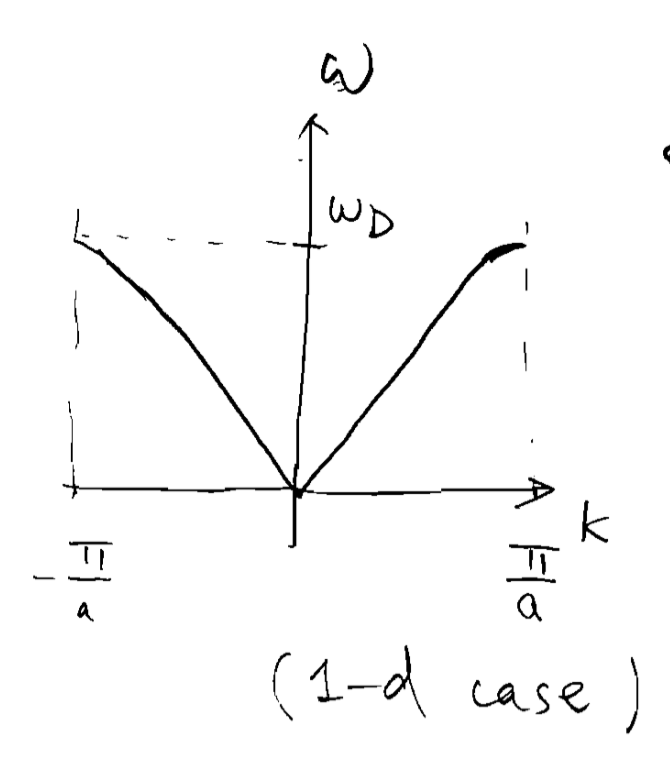
\includegraphics[width = 4.5cm]{5-2-4.png}
\end{wrapfigure}In the present model of ``elastic continuous media'', the $\omega$-integral here has no upper bound. But, in real solids, which is a discrete lattice model, the $\bf k$ integral should be taken over within the first Brillouin zone, so that the $\omega$-integral is also bounded from above at the Brillouin zone boundary. We call this upper bound of the $\omega$-integral as $\omega_D$. 
\[\sum_{\bf k} = \frac{V}{2\pi^2c^3}\int_0^{\omega_d}\omega^2d\omega \]

Since the total number of the allowed $\bf k$ points in this summation is $N$ (where $N$ is the total number of the ions), 
\[N = \sum_{\bf k} = \frac{V}{2\pi^2c^3}\int_0^{\omega_d}\omega^2d\omega = \frac{V}{2\pi^2c^3}\frac{\omega_D^3}{3} \]

From this relation, we can rewrite this into 

\[\sum_{\bf k}f(\omega_{\bf k}) = \frac{V}{2\pi^2c^3}\int_0^{\omega_D} \omega^2d\omega f(\omega) = \frac{3N}{\omega_d^3}\int_0^{\omega_D} \omega^2d\omega f(\omega) \]

Using this, the specific heat can be calculated as follows:

\[C_V = \frac{3Nk_B}{\omega_d^3}\int_0^{\omega_D} \omega^2d\omega \frac{({\beta\hbar\omega_{\bf k}})^2e^{\beta\hbar\omega_{\bf k}}}{[e^{\beta\hbar\omega_{\bf k}} - 1]^2} = \frac{3Nk_B}{(\beta\hbar\omega_d)^3}\int_0^{\beta\hbar\omega_D} dx \frac{x^4}{[e^x - 1]^2} \]
where $\beta\hbar\omega = x$. In the high temperature limit($\beta\to0$), this integral can be evaluated as 

\[C_V \approx\frac{3Nk_B}{(\beta\hbar\omega_d)^3}\int_0^{\beta\hbar\omega_D} dx \frac{x\cancel{^4}^2}{\cancel{x^2}} = \frac{3Nk_B}{(\beta\hbar\omega_d)^3}\frac{(\beta\hbar\omega_d)^3}{3} = Nk_B \]

If we further taken into account the transverse acoustic waves, the right bound side acquires another two times $Nk_B$, so that we have 

\[\lim_{T\to+\infty}C_V = \lim_{T\to+\infty}\left(C_V^{longitudinal}+C_V^{transverse}\right) = Nk_B+2Nk_B = 3Nk_B \]

In the low-temperature limit ($\beta\to0$) this integral can be also evaluated explicitly:

\[\lim_{T\to0}C_V^{longitudinal} = \frac{3Nk_B}{(\beta\hbar\omega_D)^3}\int_0^{+\infty}\frac{x^4e^x}{[e^x-1]^2}dx = \frac{4\pi^4}{5}Nk_B\left(\frac{T}{\theta}\right)^2,\quad\quad\left(\theta \equiv \frac{\hbar\omega_D}{k_B}\right) \]

which reduces to zero as a cubic function of $T$. This asymptotic behaviour is widely known as the ``Debye's $T^3$ law''. 


\section{Electron-phonon interaction} \label{se5-2}%867

So far, we have studied how the acoustic waves are second-quantized into a quadratic boson Hamiltonian. We next study the interaction between the longitudinal acoustic phonon and electron. Such an interaction is quite natural because the longitudinal acoustic waves are accompanied by the charge density modulations of positively charged ion background, which will be coupled with electron via electrostatic Coulomb interaction. To describe such interaction, let us begin with the interaction Hamiltonian between the positively charged background and electrons. 

\[H_{\text{el-p}}=\int d^3{\bf x}\int d^3{\bf x'}\frac{\rho_e({\bf x})\rho_b({\bf x'})}{|\bf x-x'|} \]

where $\rho_e({\bf x})$ denotes the electron density and $\rho_b({\bf x})$ denote the charge density of the ion background. 

\[\hat{\rho}_e({\bf x}) = -e\sum_\lambda\hat{\psi}_\lambda^\dagger({\bf x})\hat{\psi}_\lambda({\bf x}) \]
where the operator denote the electron creation/annihilation operator with spin $\lambda$ a6 $\bf x$. 

\[\begin{cases}
\hat{\rho}_b({\bf x}) &= Ze\hat{\rho}({\bf x}) = Ze(\rho_0+\delta\hat{\rho}({\bf x}))\\
&\\
\delta\hat{\rho}({\bf x}) &\equiv-\rho_0\nabla\cdot\hat{\bf d}({\bf x})
\end{cases}\]
where ``$Z$'' is the valence of the ion. 

Using this decomposition, the interaction Hamiltonian is decomposed into

\[H_{\text{el-p}} = H_{\text{el-p}}^0 + \overset{H_{\text{el-p}}^1}{\fbox{$\displaystyle\int d^3{\bf x}d^3{\bf x'}\displaystyle\frac{\rho_e({\bf x})\delta\rho_b({\bf x'})}{|\bf x-x'|}$}} \]
\begin{wrapfigure}{r}{6cm}
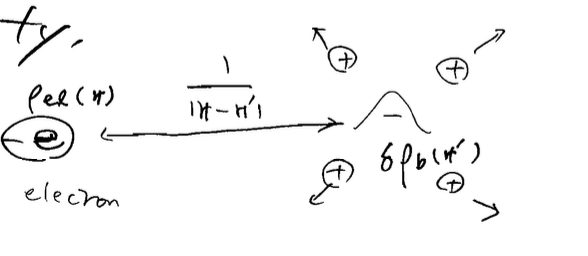
\includegraphics[width = 4.5cm]{5-2-1.png}
\end{wrapfigure}
where the first term of the right hand side was already taken into account for the purpose of ensuring the electric neutrality. 

The second term stands for the Coulomb interaction between modulated charge density of the positively charge background and electron density. In actual solids, however, the characteristic time scale of the phonon dynamics, ($\omega_D^{-1}$), is much slower than the characteristic time scale of the electron dynamics ($\epsilon_F^{-1}$). 

\[\hbar\epsilon_F\gg\hbar\omega_D \]
(phonon dynamics is much slower than the electron dynamics)

As a result, when the charge modulations is induced by the phonon dynamics, electrons in metal feels them as \uuline{static} charged impurities

\[\delta\rho_b({\bf x}):\text{ (For electrons) ``almost'' static charged impurities} \]
\begin{wrapfigure}{r}{6cm}
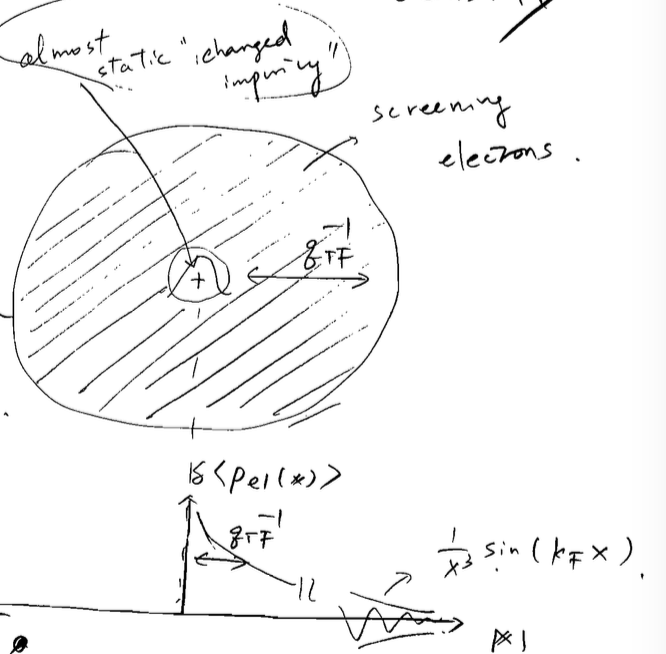
\includegraphics[width = 4.5cm]{5-2-2.png}
\end{wrapfigure}
As we have already studied in section \ref{s3-1}, such charged impurities will be immediately screened by electrons. Namely, according to the argument in section \ref{s3-1}, the static impurity induced electro density modulations. Importantly, the sum of the induced electron density is equal to minus of the charged impurity at the center. As such, the ``charged impurities'' will be completely screened, which make the interaction potential between $\delta\langle\rho_b(\bf x)\rangle$ and $\hat{\rho}_{\text{el}}(\bf x')$ here to be short-ranged potential. An explicit form of the resulting short-range interaction potential can be calculated in the following:

\[\tilde\varphi^{\text{ex}}({\bf x})=-\int\frac{e\delta\langle n({\bf x}')\rangle}{|\bf x-x'|}d^3{\bf x'}+\varphi^{\text{ex}}({\bf x}) \]

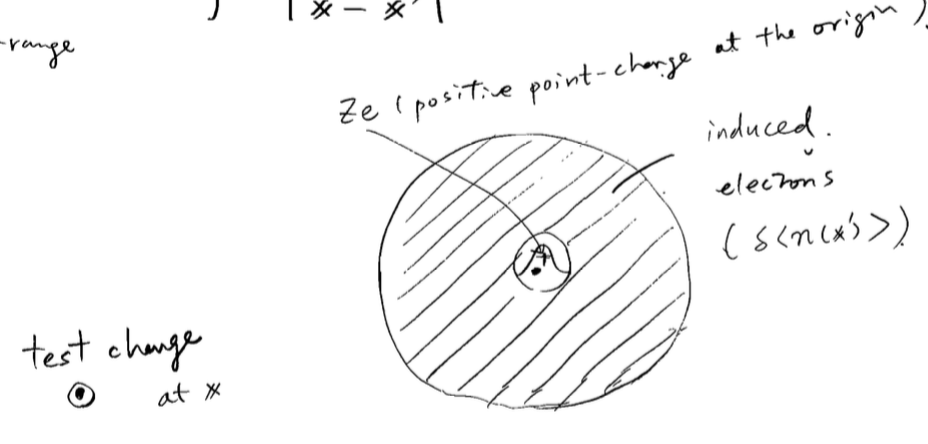
\includegraphics[width = 8cm]{5-2-3.png}

The $2-$nd term of the right hand side is the coulomb interaction between a test charge at $\bf x$ and the positive point-charge with $Ze$ charges at the origin, latter of which corresponds the ``almost static impurity'' charges associated with slow dynamics of the ion background. Such an charged impurity immediately induces screening electrons density ($\delta\langle n({\bf x})\rangle$). The first term of the right hand side is the Coulomb interactions between the induced screening electrons' density and the test charge at $\bf x$. From the argument so far, it is clear that any given electron in metals physically interacts with this positive charge via the sum of these two interactions instead of only via the latter. Within the linear response theory and within the ring-diagram approximation, we have already calculate $\delta\langle n({\bf x})\rangle$ in section \ref{s3-1}. Namely, the Fourier series of $\delta\langle n({\bf x})\rangle$ is given by

\[\delta\langle n({\bf x})\rangle =-\hbar^{-1}D^R({\bf k},0)e\varphi^{\text{ex}}({\bf x}) = -\frac{\Pi^0({\bf x},0)}{1- \Pi^0({\bf x},0)V_0({\bf k})}e\varphi^{\text{ex}}({\bf k})\]
where $e\varphi^{\text{ex}}({\bf k})$ is the Fourier series of $e\varphi^{\text{ex}}({\bf x})$ here

\[\begin{cases}
e\varphi^{\text{ex}}({\bf x}) &= \frac{Ze}{x}\\
&\\
e\varphi^{\text{ex}}({\bf k}) &= \frac{4\pi Ze}{k^2}
\end{cases}\]

As such, the Fourier series of the resulting short-range potential is readily calculated as follows:

%<- 877
%-> 881
where

\begin{align}\tag{B}\label{5B}
\hat{H}_{\text{el-ph}} = \gamma\int d^3{\bf x}\hat{\psi}_{\alpha}^\dagger({\bf x})\hat{\psi}_{\alpha}({\bf x})\hbar\varphi({\bf x})
\end{align}

with

\[\gamma = \frac{4\pi Ze^2}{q_{\text{TF}}^2}\frac{1}{c}\left(\frac{\rho_0}{M}\right)^{1/2} \]

In terms of the ele-ph coupling, our entire Hamiltonian is given by

\[\hat{H}=\hat{H}_{\text{electron-gas}}+\hat{H}_{\text{ph}}+\hat{H}_{\text{el-ph}} \]

Here $\hat{H}_{\text{el-gas}}$ was already defined in eq. \eqref{eq1.8.14}, which also includes the electron-electron interaction. $\hat{H}_{\text{ph}}$ is the quadratic boson Hamiltonian defined in eq.\eqref{5A}. $\hat{H}_{\text{el-ph}}$ was given by eq.\eqref{5B}. Even though we ignore the electron-electron Coulomb interaction in the first term, this Hamiltonian is still essentially quantum many-body problem, because of the coupling between phonon \& electron. In order to highlight the electron-phonon interaction, let us for a while ignore the electron-electron Coulomb interaction and construct zero-temperature perturbation theory for this coupled-field theory. 

Namely, our Hamiltonian is

\[\hat{H} = \sum_{\bf k,\alpha}(\epsilon_{\bf k}-\mu)a^\dagger_{\bf k,\alpha}a{\bf k,\alpha} + \sum_{\bf k}\hbar\omega_{\bf k}c_{\bf k}^\dagger c_{\bf k} + \gamma\int d^3{\bf x}\hat\psi_\alpha^\dagger({\bf x})\hat\psi_\alpha({\bf x})\hat\varphi_\alpha({\bf x}) \]

where electron fields with spin index $\alpha$ are Fourier transformed with a normalization which is a bit different from what we used so far

\[\hat\psi_\alpha^\dagger({\bf x}) = \sum_{\bf k}\frac{1}{\sqrt{V}}e^{-i\bf k\cdot x}a^\dagger_{\bf k,\alpha} \]
\[\hat\psi_\alpha({\bf x}) = \sum_{\bf k}\frac{1}{\sqrt{V}}e^{i\bf k\cdot x}a{\bf k,\alpha} \]
which make the momentum integral to be a single discrete summation

\[\hat\varphi({\bf x})=\sum_{\bf k}\sqrt{\frac{\hbar\omega_{\bf k}}{2V}}\left[c_{\bf k}e^{i\bf k\cdot x}+e_{\bf k}^\dagger e^{-i\bf k\cdot x}\right] \]
\dotfill
\ 

As I explained already, the acoustic phonon has an upper bound for its frequency, so that I will put a step function within this sum, to take into account this effect. 
\[\hat\varphi({\bf x})=\sum_{\bf k}\sqrt{\frac{\hbar\omega_{\bf k}}{2V}}\left[c_{\bf k}e^{i\bf k\cdot x}+e_{\bf k}^\dagger e^{-i\bf k\cdot x}\right] \theta(\omega_D-\omega_{\bf k}) \]
\dotfill

\ 

In the coupled field theory, we clearly can define two Green's functions. One is the Green's function for electrons. The other is the Green's function for phonons. 


%<- 885

%-> 889
Feynman's rule for these two Green's functions can be derived exactly in the same way as we did for electron-electron interaction. I will summarize the Feynman's rule in the \uline{momentum space} representation. 

First of all, the Wick's theorem suggests that the $2n$-th order in $\hat{H}_1$ contribute to these Green's function, where $n$ is integer. For the $2n$-th order contribution to $G({\bf q},q_0),\ D({\bf q},q_0)$, the rule is as follows. 

\begin{wrapfigure}{l}{4cm}
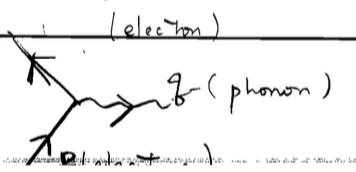
\includegraphics[width = 4cm]{5-2-l5.png}
\end{wrapfigure}
\noindent (a) Construct all topologically distinct Feynman diagrams, where the basis vertex is composed of two electron lines and one phonon(electron) line meeting at the vertex. 

\noindent (b) Assign $G_{\alpha\beta}^0(p)$ for each electron line and assign $D^0(q)$ for each phonon line, where the non-interacting electron Green's function is given by the same function as before

\[G_{\alpha\beta}^0({\bf q},q_0) = \delta_{\alpha\beta}\left[\frac{\theta(|{\bf q}|-k_F)}{q_0-\epsilon_{\bf q}/\hbar+i\eta} + \frac{\theta(k_F - |{\bf q}|)}{q_0-\epsilon_{\bf q}/\hbar-i\eta}\right] \]

The non-interacting phonon Green's function is defined in the real space as follows 

\[iD^0({\bf x},t;{\bf x'},t') = \langle vac|\mathcal{T}[\hat\varphi_I({\bf x},t)\hat\varphi_i({\bf x'},t')]|vac\rangle \]
where

\[\hat\varphi_I({\bf x},t) = e^{iH_0t/\hbar}\hat\varphi_I({\bf x})e^{-iH_0t/\hbar} = \sum_{\bf k}\sqrt{\frac{\hbar}{2V}}\left[c_{\bf k}e^{i{\bf k\cdot x} - i\omega_{\bf k}t} + c_{\bf k}^\dagger e^{-i{\bf k\cdot x} + i\omega_{\bf k}t}\right] \cdot\theta(\omega_{\bf k} - \omega_D)\]

\[\begin{split}
iD^0({\bf x},t;{\bf x'},t') &= \theta(t-t')\langle vac|\hat\varphi_I({\bf x},t)\hat\varphi_I({\bf x'},t')|vac\rangle + \theta(t'-t)\langle vac|\hat\varphi_I({\bf x'},t')\hat\varphi_I({\bf x},t)|vac\rangle\\
&= \theta(t-t')\sum_{\bf k}\frac{\hbar\omega_{\bf k}}{2V}e^{i{\bf k\cdot(x-x')}-i\omega_{\bf x}(t-t')}\langle vac|\cancel{c_{\bf k}c_{\bf k}^\dagger}|vac\rangle\theta(\omega_D-\omega_{\bf k})\\
&\ \ \  + \theta(t-t'){\color{red}{\sum_{\bf k}\frac{1}{2V}}}\hbar\omega_{\bf k}e^{-i{\bf k\cdot(x-x')}+i\omega_{\bf x}(t-t')}\langle vac|\cancel{c_{\bf k}c_{\bf k}^\dagger}|vac\rangle\theta(\omega_D-\omega_{\bf k})\\
&\quad\quad\quad\quad\quad\int \frac{d^3\bf k}{(2\pi)^3}\\
\end{split} \]

By defining its Fourier series as in the electron Green's function:

\[=\int \frac{d^3\bf q}{(2\pi)^3}\int \frac{d q_0}{2\pi}e^{i{\bf q(x-x')}-iq_0(t-t')}iD^0({\bf q},q_0) \]

we have

\[D^0({\bf q},q_0)=\frac{\hbar\omega_{\bf q}}{2}\left(\frac{1}{q_0\omega_{\bf q}+i\eta}-\frac{1}{q_0+\omega_{\bf q}-i\eta}\right)\times\theta(\omega_D-\omega_{\bf q}) \]

\begin{wrapfigure}{l}{3cm}
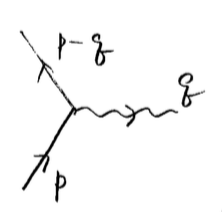
\includegraphics[width = 3cm]{5-2-l6.png}
\end{wrapfigure}
\noindent (c) We impose the conservation of the momentum and energy (frequency) at each vertex

\noindent (d) Integrate all the internal momentum and frequency as $\displaystyle\int d^3{\bf q}\int dq_0$

\noindent (e) Include a factor of

\[i^n\left(\frac{\gamma}{\hbar}\right)^{2n}\left(\frac{1}{(2\pi)^4}\right)^n\cdot(-1)^F \]
where $F$ is the number of the electron loop in a given Feynman diagram. 

\noindent (f) Discards all Feynman diagrams which have subunits connected to the rest of the diagrams by only one phonon line. 

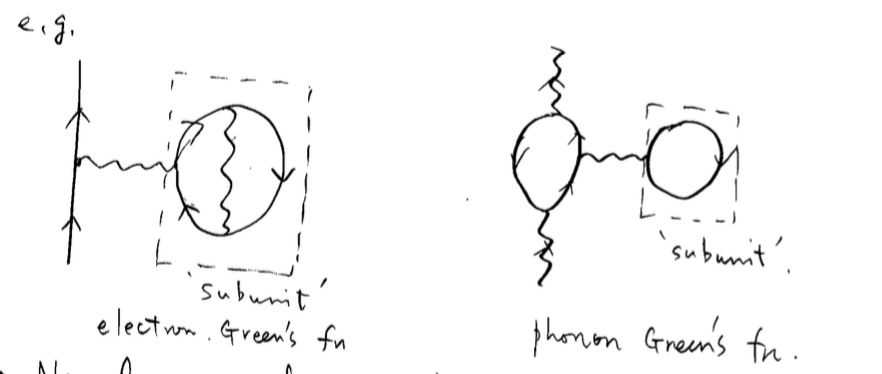
\includegraphics[width = 7cm]{5-2-l7.png}

These Feynman's rules are applicable for both electron's Green's function \& phonon's Green's function. Equivalent electron-electron interaction and BCS (Bardeen-Cooper-Schrieffer) Hamiltonian. 

Comparing this Feynman's rule for the electron-phonon coupled system and the Feynman's rule for interacting electron system (given in section \ref{S2-5}), one can realize the ``equivalence between these two different quantum many-body systems. 

\newpage
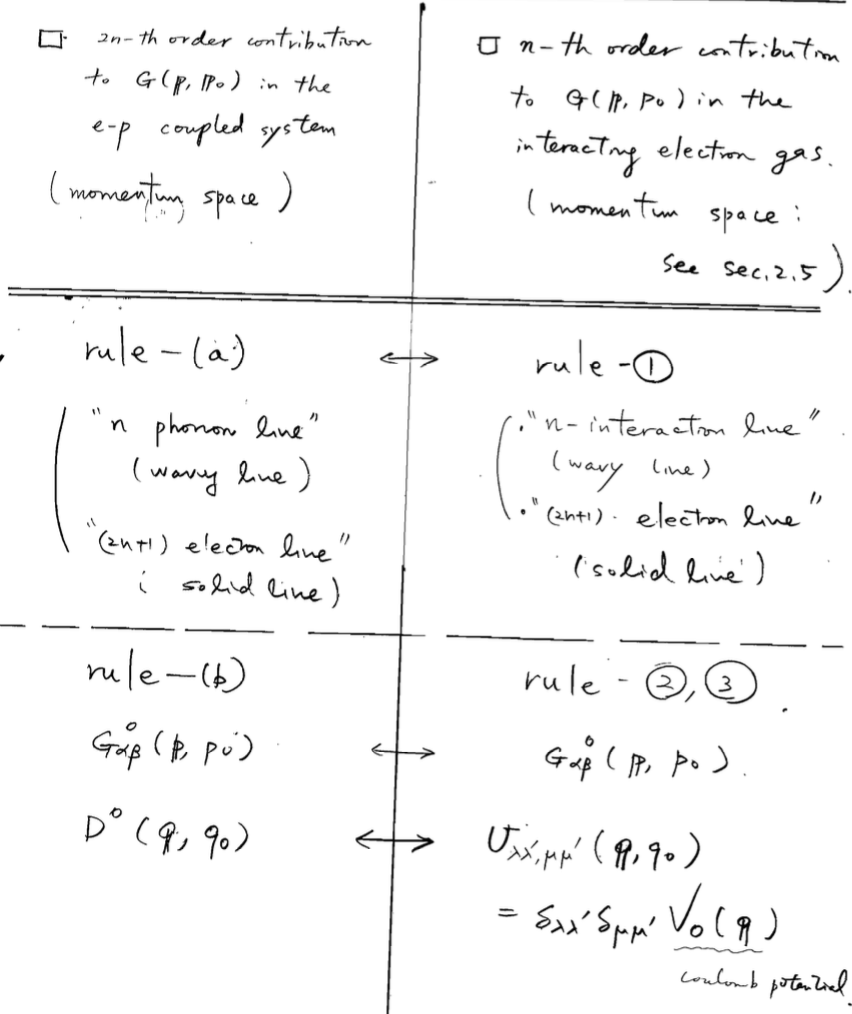
\includegraphics[width = 15cm]{5-2-l4.png}\\
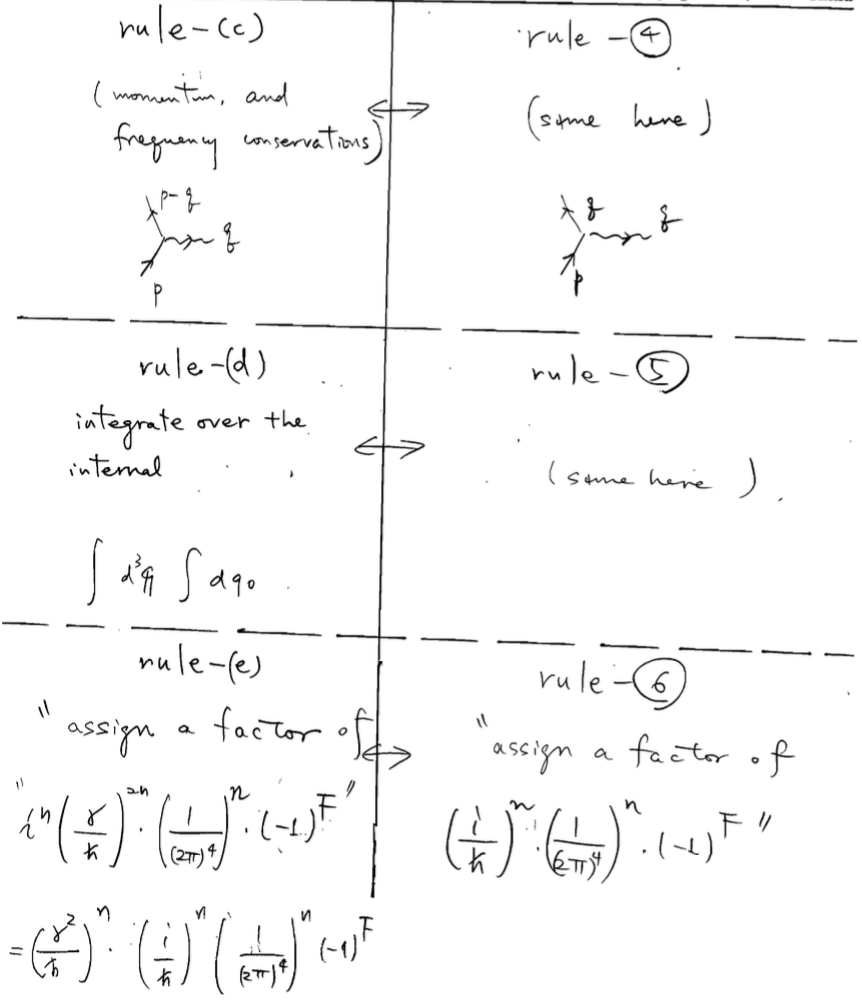
\includegraphics[width = 15cm]{5-2-l3.png}
\newpage
This one-to-one correspondence suggests that, electron Green's function in e-p coupled system becomes exactly same as the electron's Green's function in an interacting electron system, where the interaction potential is given by the non-interacting phonon propagator: Namely the interaction potential is spin-independent and frequency dependent and is given by this

\[\begin{split}
\tilde{U}_{\lambda\lambda',\mu\mu'}({\bf q},q_0)&\equiv\frac{\gamma^2}{\hbar}D^0({\bf q},q_0)\delta_{\lambda\lambda'}\delta_{\mu\mu'}\\
&=\frac{\gamma^2}{\cancel\hbar}\frac{\cancel{\hbar}\omega_q}{2}\left(\frac{1}{q_0-\omega_{\bf q}+i\eta} - \frac{1}{q_0+\omega_{\bf q}-i\eta}\right)\theta(\omega_D-\omega_q)\delta_{\lambda\lambda'}\delta_{\mu\mu'}\\
&=\gamma^2\frac{\omega_q^2}{q_0^2-(\omega_{\bf q}-i\eta)^2}\theta(\omega_D-\omega_{\bf q})\delta_{\lambda\lambda'}\delta_{\mu\mu'}
\end{split} \]

where this factor $\gamma^2/\hbar$ comes from this addition factor. In the static limit, the interaction potential become attractive

\[ U_0({\bf q},0) = -\gamma^2\theta(\omega_D-\omega_{\bf q})\delta_{\lambda\lambda'}\delta_{\mu\mu'}\]

Since we are interested in the long wave length regime of the phonon, for ${\bf q}\ll k_F$, $\omega_{\bf q} = e{\bf q} \ll ck_F\approx\omega_D$, $\omega_{\bf q}$ is much smaller than the Debye frequency, so that we can simply replace this by a negative valued constant function in $\bf q$:

\[U_0({\bf q},0)\simeq -\gamma^2\quad\text{for }{\bf q}\ll k_F \]

This means that the equivalent electron-electron interaction becomes an attractive delta function

\[V_{\text{eq}}({\bf x}) = \int\frac{d\bf q}{(2\pi)^3}e^{i\bf q\cdot x}U_0({\bf q},0) = -\gamma^2\delta^3(\bf x) \]

As we will see in the next chapter, this attractive electron-electron interaction results in superconductivity. Remember that the equivalent interaction potential will become repulsive when the energy transfer between two electrons are greater than $\omega_D$

\begin{wrapfigure}{r}{5.5cm}
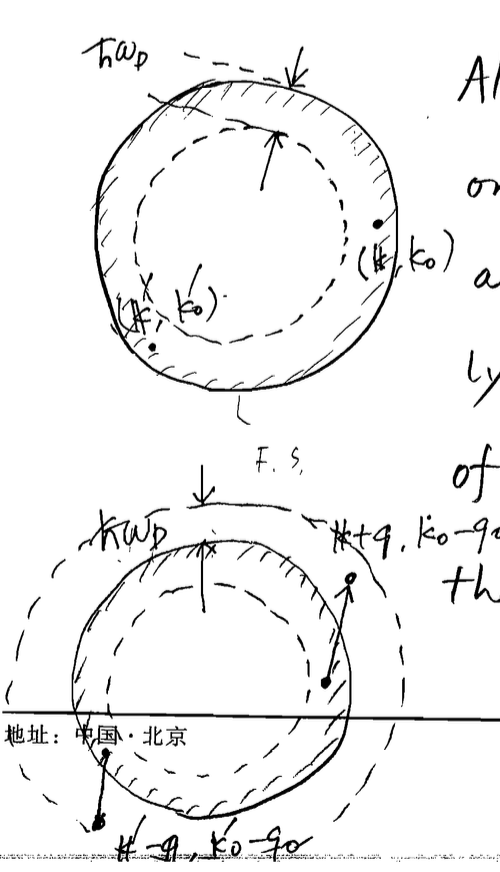
\includegraphics[width = 4.5cm]{5-2-l1.png}
\end{wrapfigure}
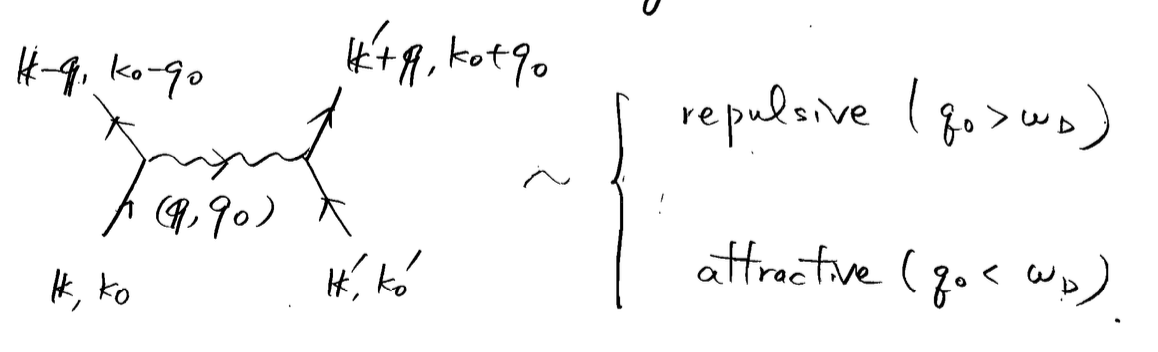
\includegraphics[width = 8cm]{5-2-l2.png}

In the non-interacting ground state where electrons form a Fermi sea, $U_0({\bf q},q_0)$ can be attractive only for those electrons lying within an energy shell of the thickness $\hbar\omega_D$ belong the Fermi surface. Also, $U_0({\bf q},q_0)$ is attractive only when these two electrons are scattered into the states lying with an energy shell of the thickness $\hbar\omega_D$ above the Fermi surface. 

The electron gas model with this attractive interaction potential with the delta function form is called as the BCS Hamiltonian, which is the starting Hamiltonian for the microscopic theory of superconductivity in metal. 

\[\hat{K} = \int d^3{\bf x}\hat{\psi}^\dagger_\alpha({\bf x})\left[-\frac{\hbar^2\nabla^2}{2m}-\mu\right]\hat{\psi}_\alpha({\bf x}) - \frac{g}{2}\int d^3{\bf x} \hat{\psi}^\dagger_\alpha({\bf x})\hat{\psi}^\dagger_\beta({\bf x})\hat{\psi}_\beta({\bf x})\hat{\psi}_\alpha({\bf x})\]

with

\begin{align}\tag{C}
g\equiv\gamma^2\equiv\frac{16\pi^2 Z^2 e^4}{q_{\text{TF}}^4}\frac{1}{c^2}\left(\frac{\rho_0}{M}\right) \end{align}



